%DataLogging
%%swith to your GitHub not done yet.
\chapter{DataLogging}
It today's lab, we are going to measure temperature. We will use a transducer that turns temperature (energy of the air molecules around us) into a voltage. So we are still learning to use transducers. But instead of concentrating on validating a physical model for temperature, we are going to concentrate on building an independent system to measure temperature, one that doesn't have to be connected to our computer.

Often we need to have a data collection device that can operate far from our computer, but still save data for later use. For example, if you were to launch your Arduino-instrument on a high altitude balloon.

Today we all need to be able to have our Arduino collect data and save it with no computer attached. We will do this using a shield. An Arduino shield fits over the top of your Arduino, connecting to the necessary pins to do its job. The other pins are still available to use for other measurements. 

\begin{figure}[h!] 
	\centering
	\caption{Top of a prototyping shield}
	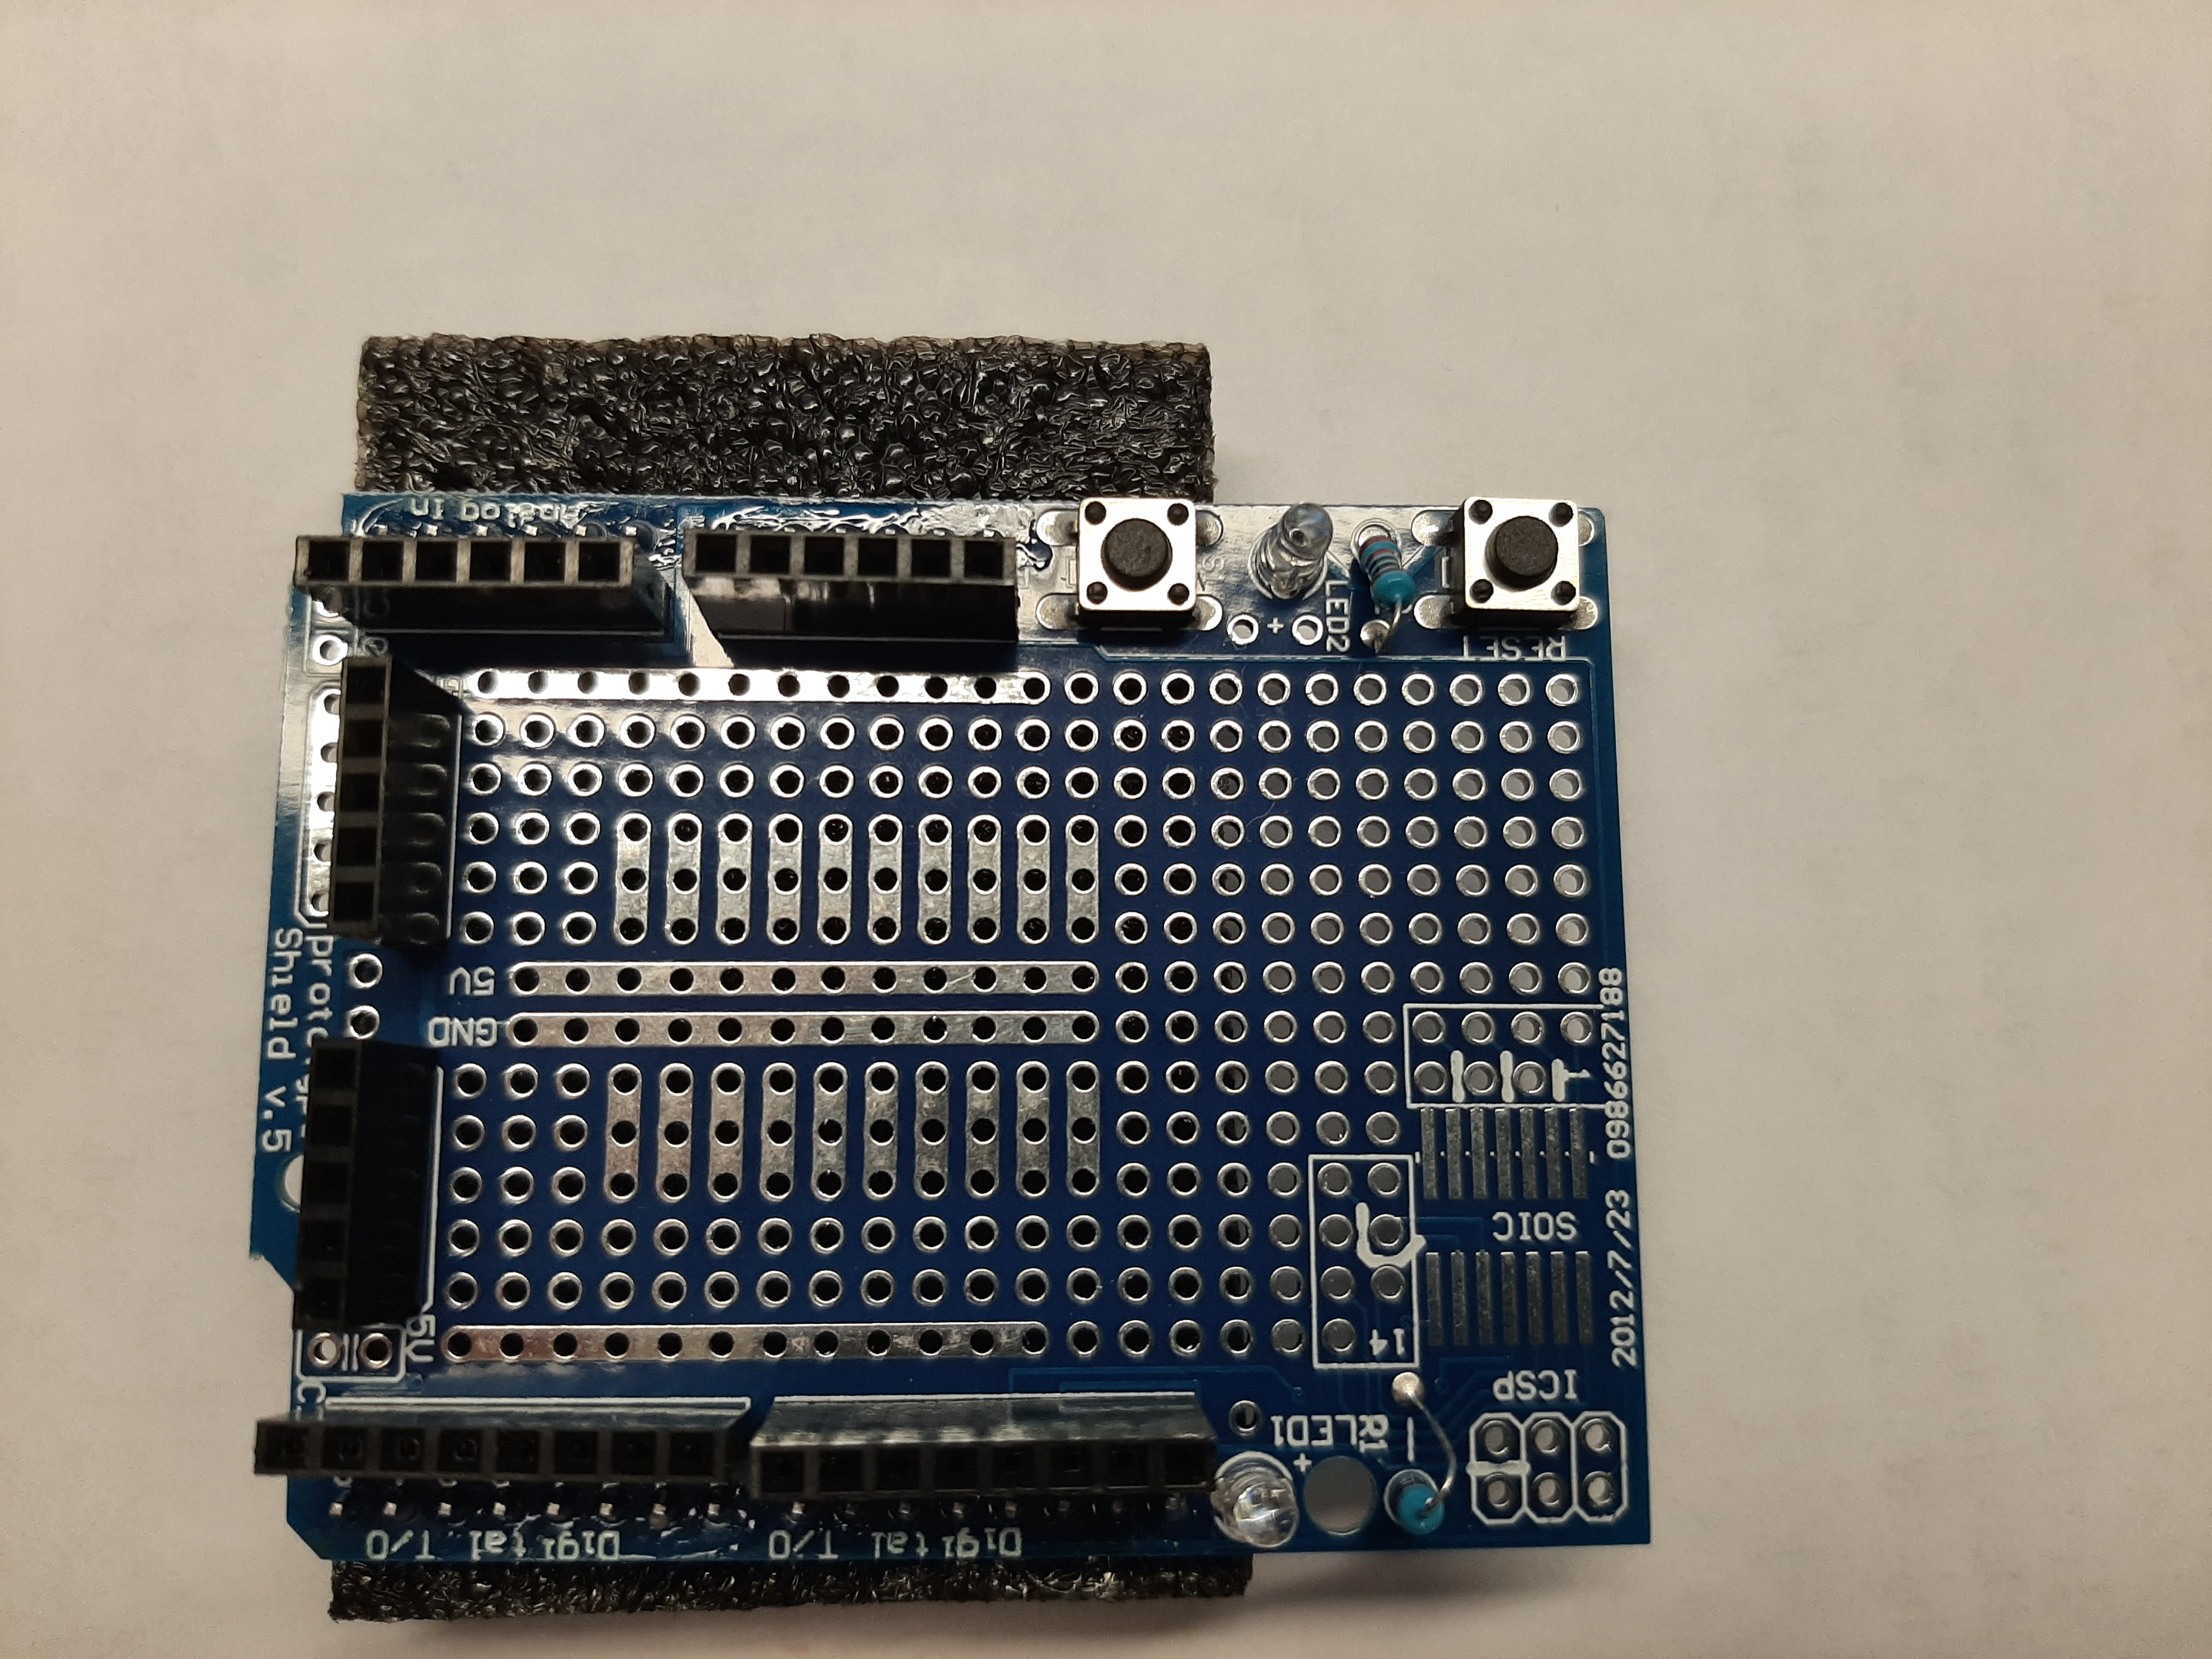
\includegraphics[width=3.614in,height=2.3981in]{20200309_133406}
\end{figure}

\section{Arduino Shields}
	Arduino shields are a simple way to add specific functionality to your Arduino. There are many different shields with many different features. Some shields have additional integrated circuit (IC) chips on them that can add additional computational power.  Others are extremely simple and are designed so you can have a more solid electrical connections with your experiment.  The previous figure and the next figure are the top and bottom of an example of a simple prototyping shield.

	\begin{figure}[h!] 
		\centering
		\caption{Bottom of a prototyping shield}
		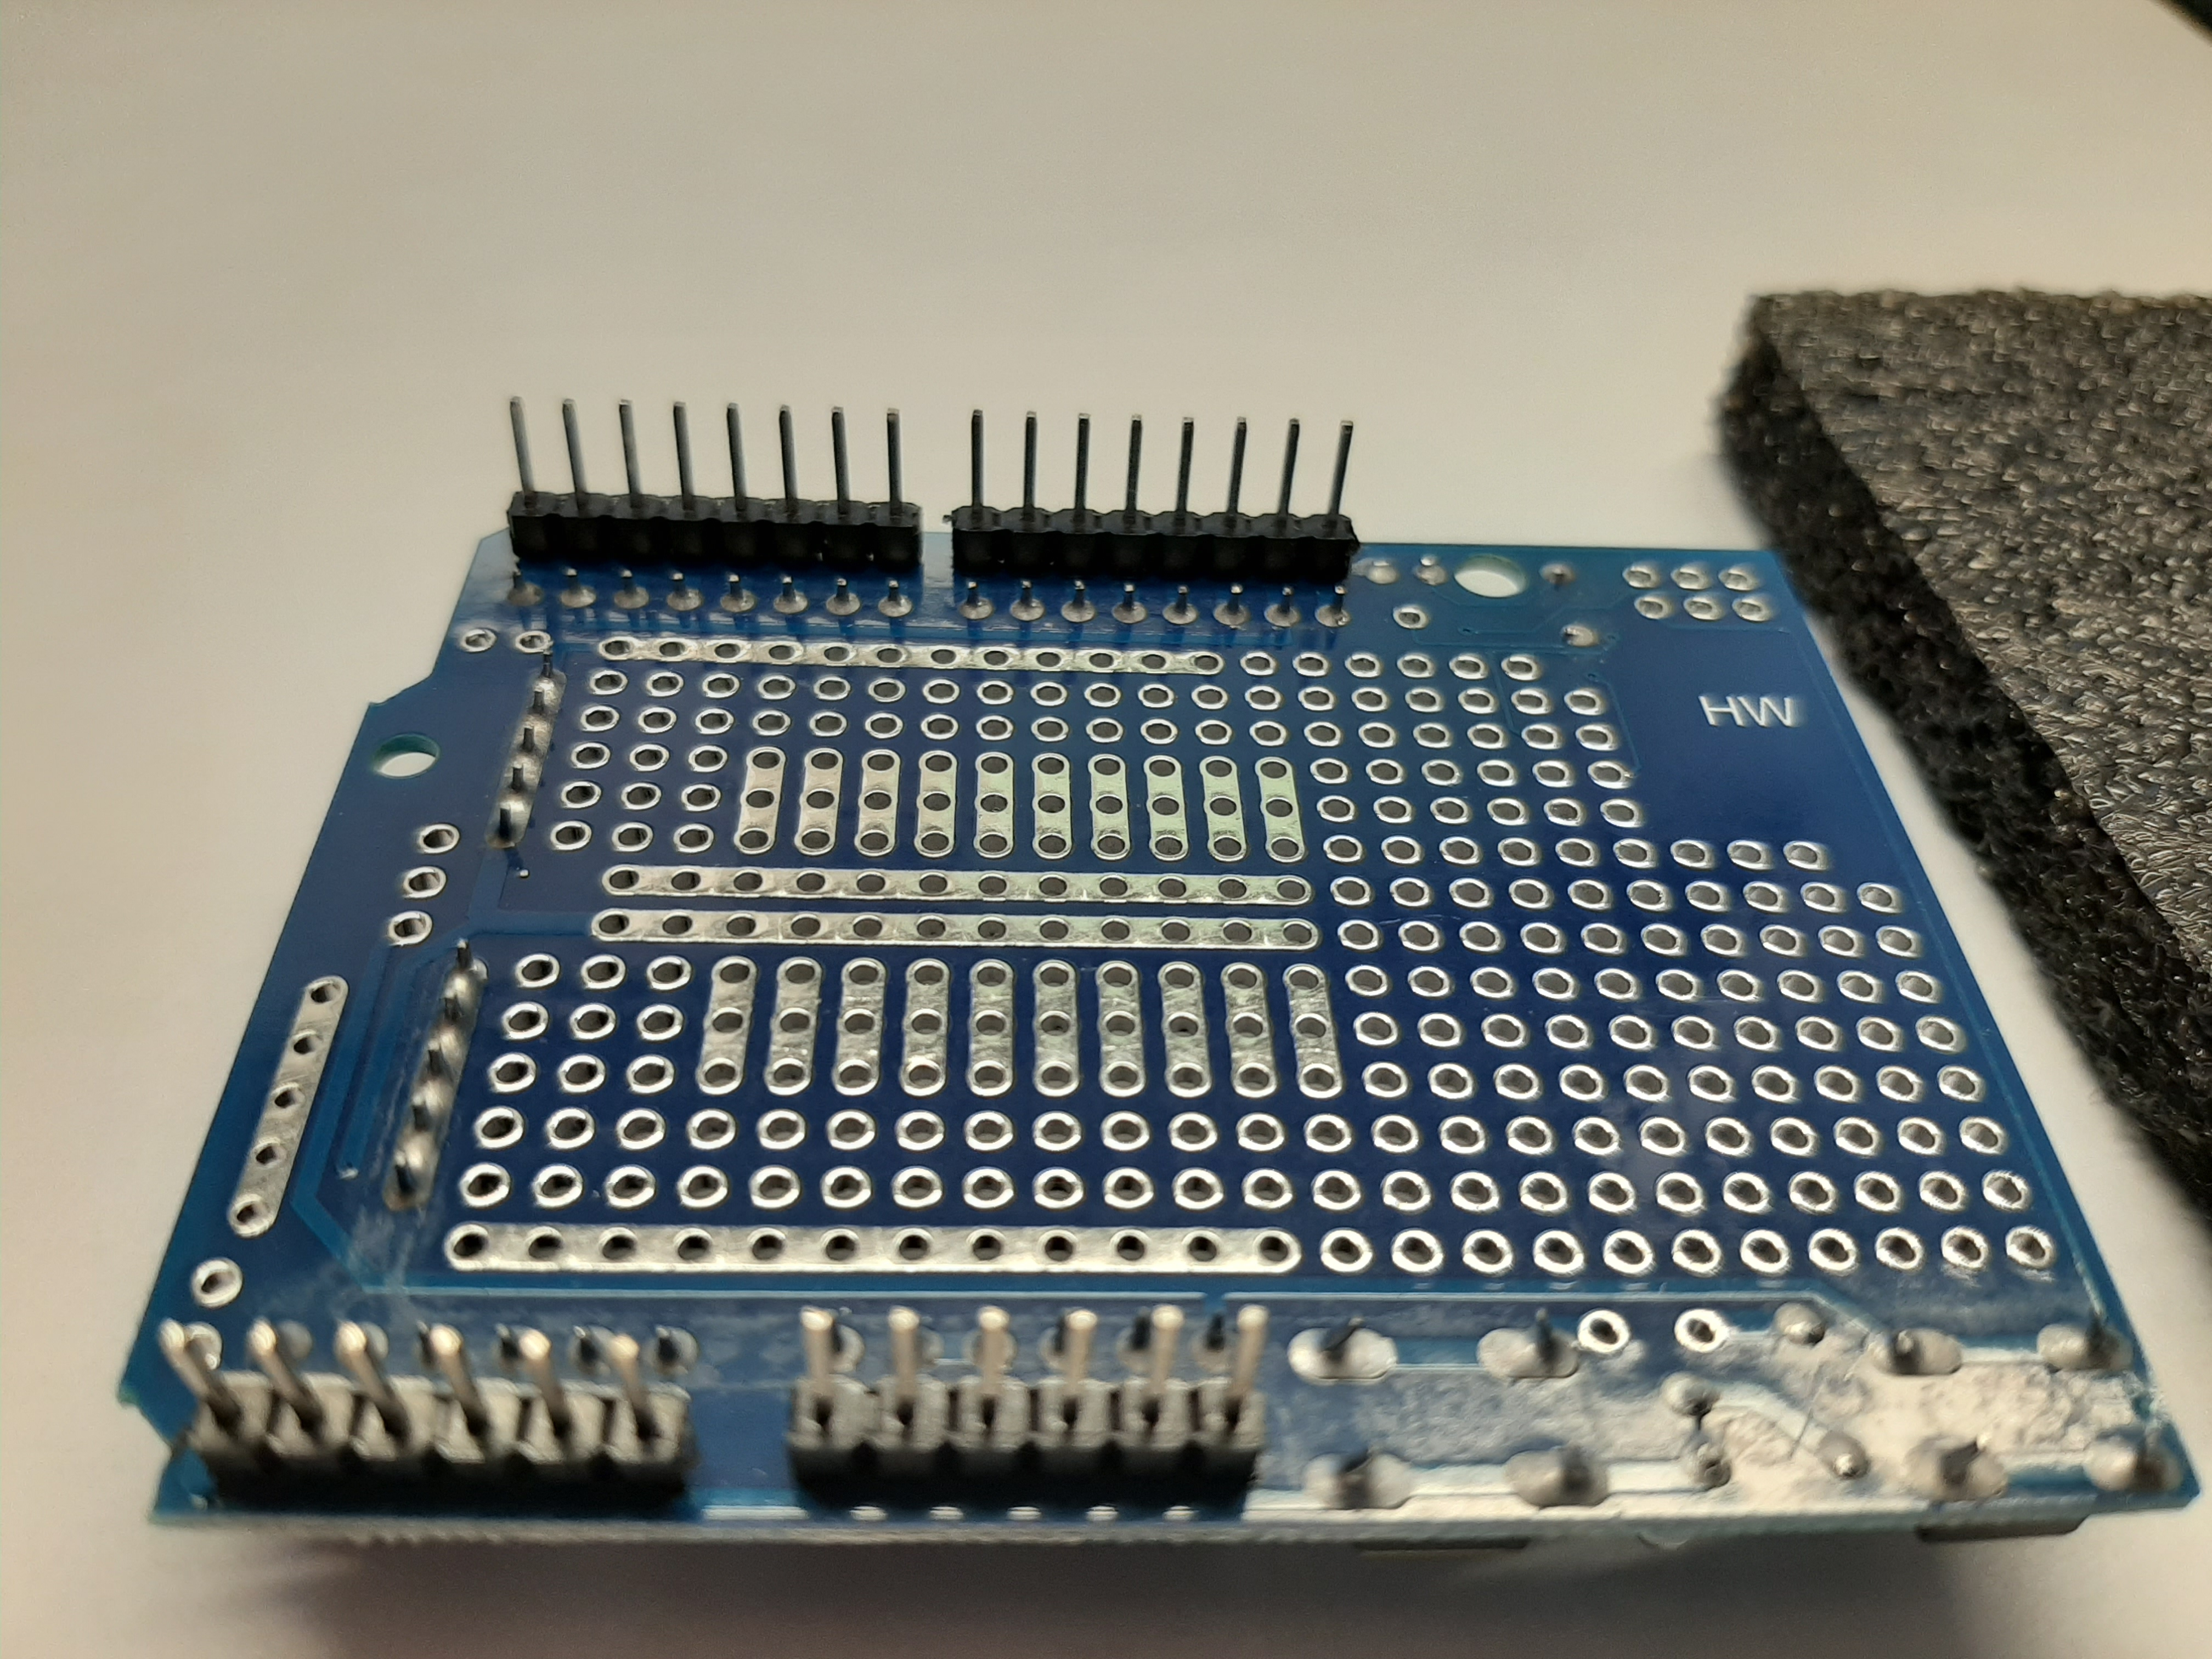
\includegraphics[width=3.614in,height=2.3981in]{20200309_133450}
	\end{figure}
	
	Notice the long wire pins on the bottom. These are designed to be plugged in directly into the Arduino. When not in use these should be pushed into the conductive foam. This will not only protect them from getting bent, but will also protect the electrical circuits on the shield from static shocks.
	
	Many shields are compatible with other shields such that they can be stacked onto each other. This will depend on what pins each shield is using and on the physical placement of both the bottom and top pins.
	
	Because shields are designed for a specific functionality the manufactures will often provide example code that utilizes those features. This code can then be modified and/or combined with other code to get your Arduino to do what ever you want. While working with shields be aware of the pins that the shield is using. So you don't interfere with its operation use other pins for your experiments.

\section{Data Logger Shield}
	Data logging is one of the most important parts of any experiment. Data for many experiments often depend on time. The data logger shield allows us to not only save the data to an SD card but we can also save the time along with it. This is because it has a built in real time clock(RTC). The data logger shield is shown in the next figure.
	
	Take a close look at the figure \ref{Data_Logger}. You will notice that the SD card slot (right next to the words ``Data logger Shield'') is close to an integrated circuit (IC). That IC (a black rectangle) controls the SD card. 
	
	There is also a battery holder. It has a battery in it, but the image also shows a piece of blue paper covering both sides of the battery. This is for shipping so that the battery isn't drained while not in use. The battery is needed for the real time clock. So that it keeps time even if there is no other power to the board. 
	
	But why do we need a clock on our datalogger?  Often we just need to know what time the data was collected.  But more importantly, we might wish to compare our data to data collected on another instrument. If we know what time the data points were gathered, the comparison is easier.  For one example, suppose I am measuring the temperature from the ground to $30km$. My instrument measures temperature (like the one we will build today) but I want to know the temperature as a function of altitude.  I will need an altimeter to collect data along with my temperature instrument.  To match up the data from my instrument and the altimeter, both can record the time for each data point and then I can match the times from my temperature data and the times from the altitude data to get my temperature as a function of altitude.  Our BYU-I High Altitude Research Team uses this method for most of their instruments.
	
	On our data logger shield the electronics for the RTC are right next to the battery. Note the smaller IC and the silver cylinder. The cylinder holds a small quartz crystal tunning fork that keeps oscillating. These oscillations are counted by the IC and are used to keep time. 
	
	\begin{figure}[h!] 
		\centering
		\caption{Top of Data Logger Shield}
		\label{Data_Logger}
		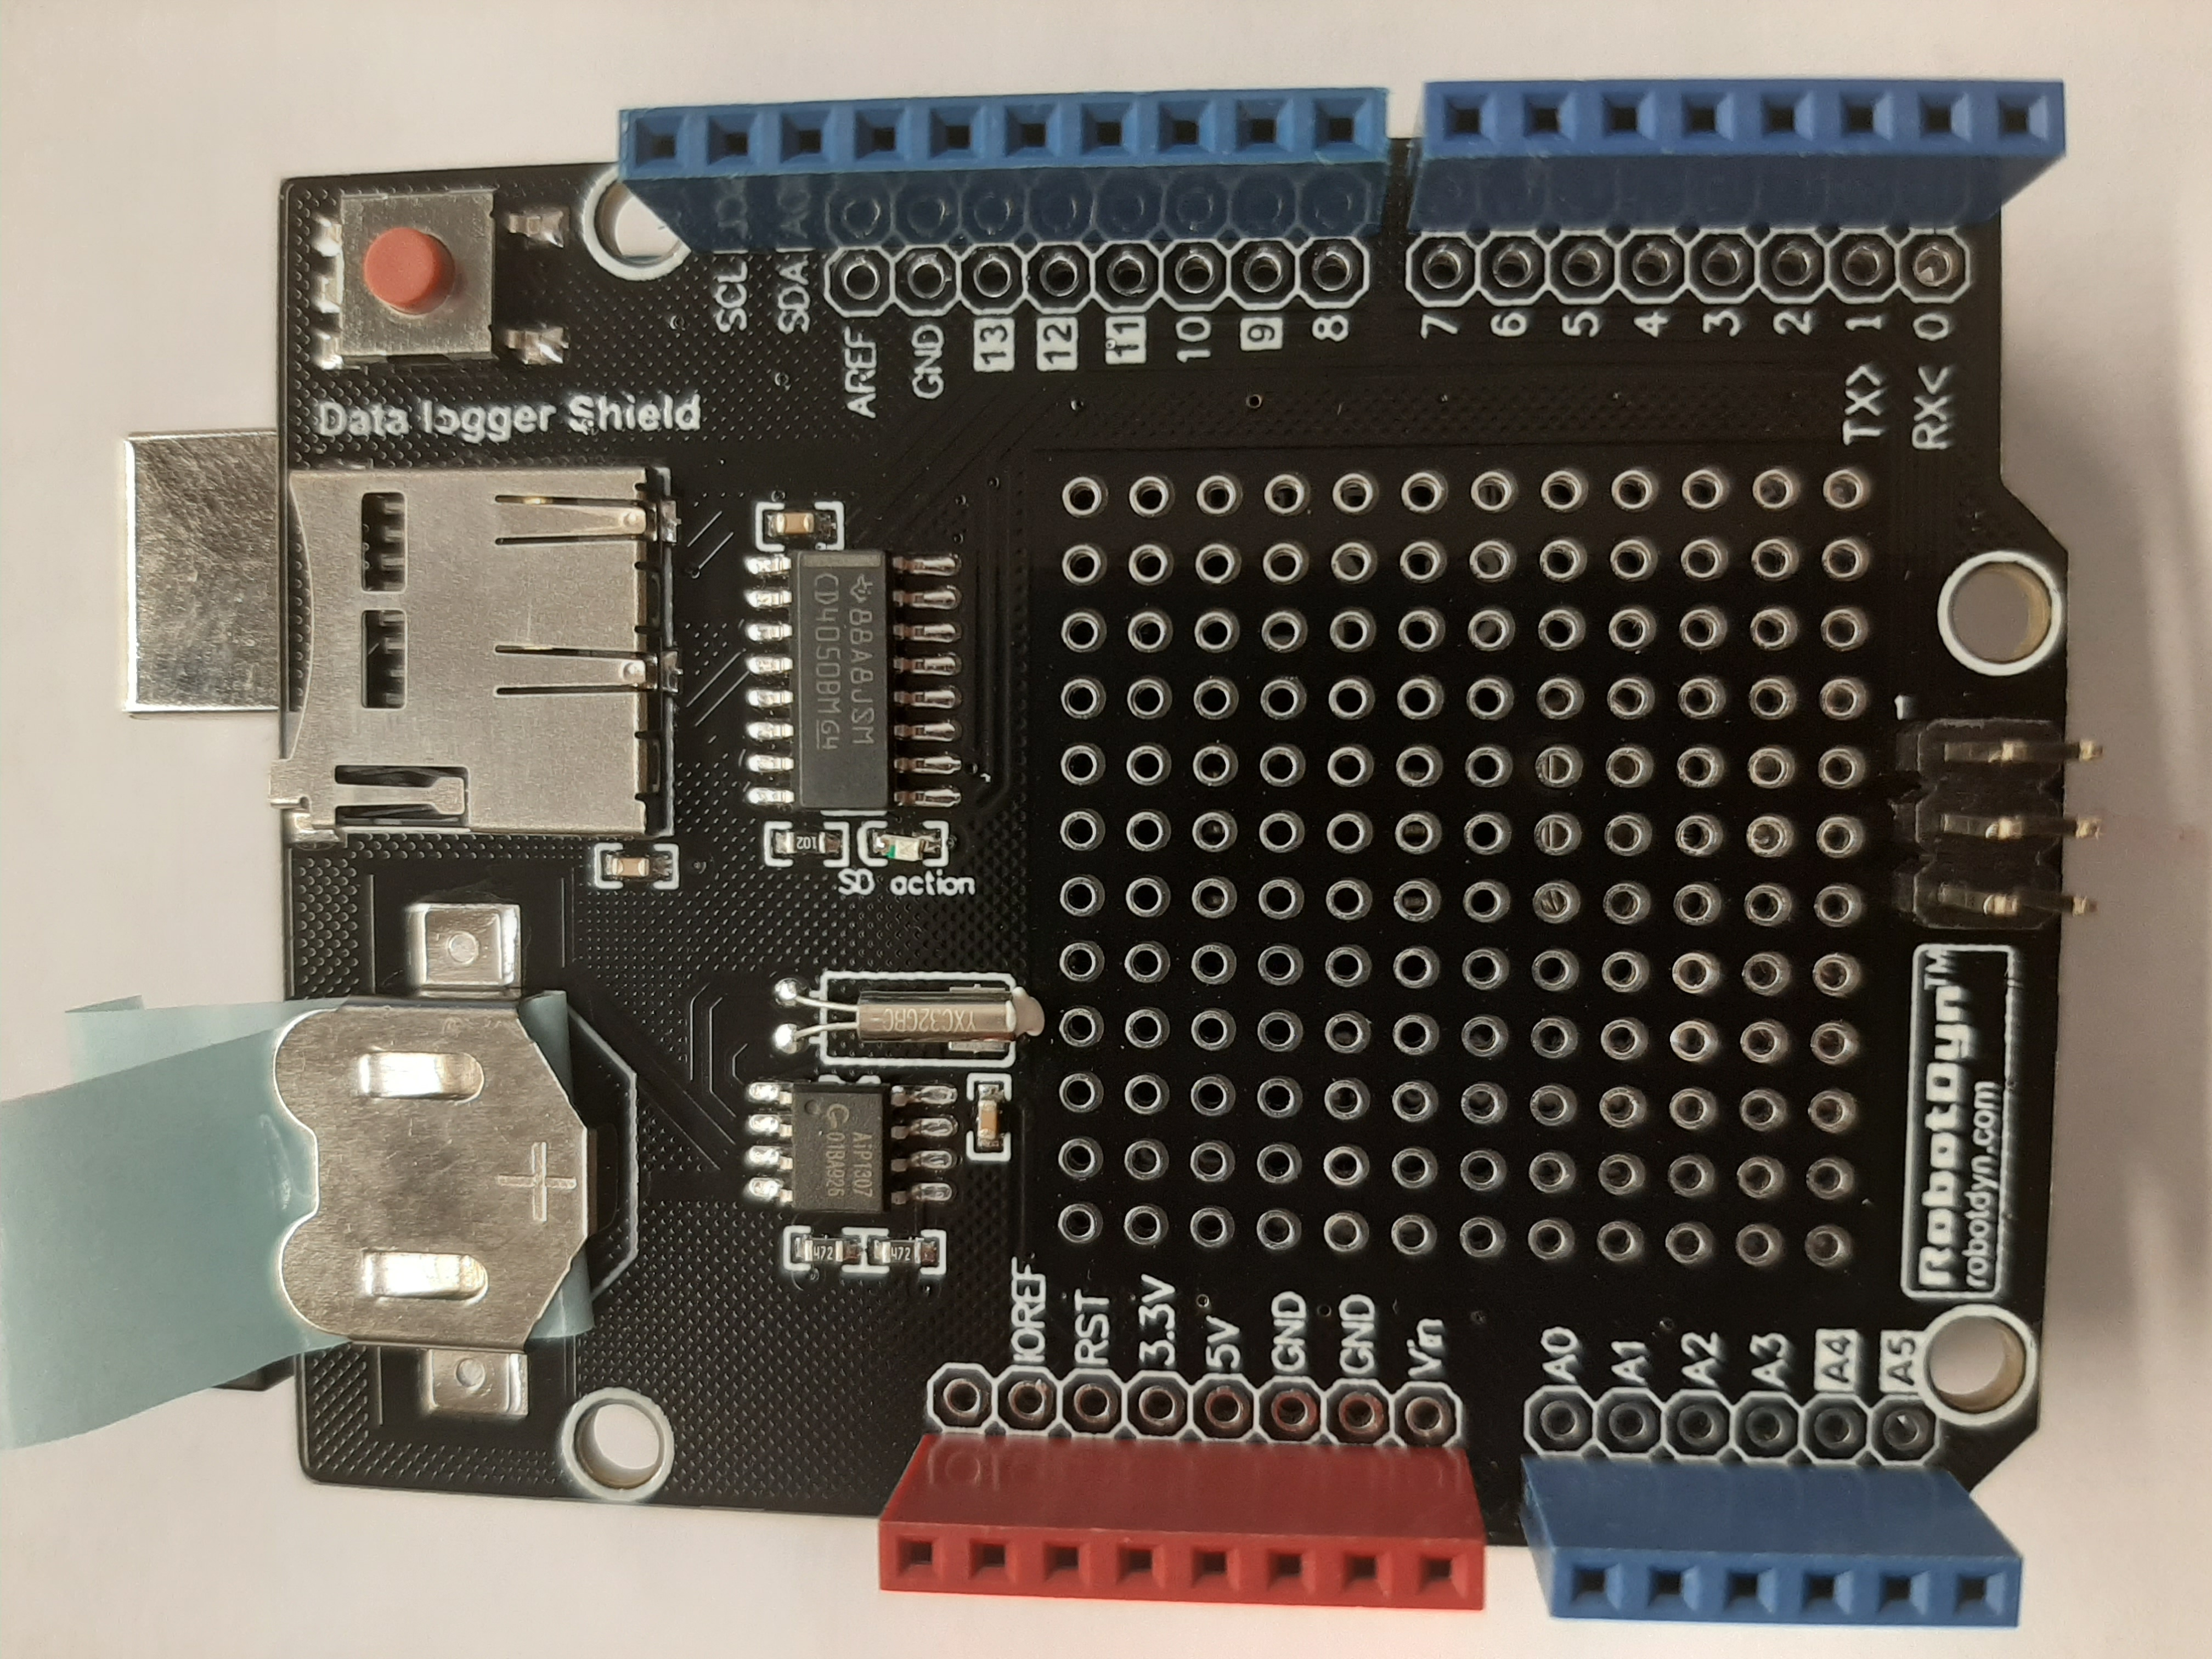
\includegraphics[width=3.614in,height=2.3981in]{20200310_110036}
	\end{figure}
	
	Just like on your Arduino the pins are all labeled. But notice that some of the pins are labeled with a white square and a back number. These pins (A4, A5, 9,11,12 and 13) are the pins that the shield uses for its functions. Make sure that your experiment doesn't use these pins. Pins A4 and A5 are used for the RTC and pins 9,11,12 and 13 are used for the SD card. The bottom of shield gives additional labels to these pins that describe their function. 



\section{Set up}
	The Data Logger shield uses a library. To get that library follow these steps in the Arduino software.
	
	\begin{enumerate}
		\item Under "Tools" go to ``Manage Libraries ...''
		\item Search for ``RTClib''
		\item Find the library by Adafruit and install it.
	\end{enumerate}

    The first time the software is run on the Arduino with the Data Logger shield the RTC needs to be set.  Pull out the paper that keeps the battery from contacting  and put the battery back (if the paper is still there). Then upload the code below. Check the serial monitor. If it says that the ``RTC has not been set!'' or if the date and time are incorrect then you will need to remove the comment back slashes on the line 
    
    \begin{lstlisting}[language=Arduino]
   		 rtc.adjust(DateTime(2014, 1, 21, 3, 0, 0));
    \end{lstlisting}
    
    \noindent but change the numbers to match the current date and time. Then upload the code again. This will set the clock. This only needs to be done once, as the battery will keep time from then on. So put the comment back slashes back in and upload the code again.

%%%%%%%%%%%%%%%%%%%%%%%%%%%%%%%%%%%%%%%%%%%%%%%%%%%%%%%%%%%%%%%%%%%%
\href{https://raw.githubusercontent.com/rtlines/IntermediateLabPH250/main/Code/DataLog.ino}{Download here}
%%%%%%%%%%%%%%%%%%%%%%%%%%%%%%%%%%%%%%%%%%%%%%%%%%%%%%%%%%%%%%%%%%%%
    \lstinputlisting[language=Arduino]{Code/DataLog.ino}


The code above saves random data to the SD card. When you have it working check to see that the data file is on the SD card by putting the SD card in your computer and opening the file.  

Of course, we don't want random data. You will need to modify the code such that it saves the temperature. But just getting the time information to safe to the SD card is a great first step!

Before we go on to add the sensor, spend a few moments looking at the example code.  Notes that at the end there are some special functions that do things like initialize the RTC and the SD card reader.  These are used by the setup() function to get things working. You should not have to change these much.  But do note that they need to be part of your code for the datalogger shield to work.

Also notice up at the top of the example code there are more include statements and some special variables.  Like the 

 \begin{lstlisting}[language=Arduino]
	RTC_DS1307 rtc;
\end{lstlisting}
line or the 
 \begin{lstlisting}[language=Arduino]
	SD_PIN = 9; 
\end{lstlisting}
line. These are also needed by the datalogger. So we will have to include them in our codes. 

One strategy might be to start with the example code so we are sure we have all of these new parts included.

\section{Adding in your sensor}
So now that you have your time being recorded (plus a random number) we want to make the modification so that our datalogger is recording temperatures.  We will start with the thermistor from your Arduino kit. This termistor was produced by the Elegoo company that made your kit.  It might be tempting to google termistors to find out how to use it. \textbf{But don't do this! } This thermistor was made by a specific company, and we need to go to that specific company to learn how to use it.  We might find similar instructions for other thermistors from other companies, but they almost certainly won't be right for our specific thermistor.  We need the Elegoo instructions. 

And these instructions are hidden on the CD that came with your kit.  But who has a CD player in their computer anymore?  To get around this we will go to the Elegoo web site and download their instructions. Here is a link:

\begin{center}
%%%%%%%%%%%%%%%%%%%%%%%%%%%%%%%%%%%%%%%%%%%%%%%%%%%%%%%%%%%%%%%%%%%%
 \href{https://www.elegoo.com/products/elegoo-uno-project-super-starter-kit}{Link to Elegoo website}
%%%%%%%%%%%%%%%%%%%%%%%%%%%%%%%%%%%%%%%%%%%%%%%%%%%%%%%%%%%%%%%%%%%%
\end{center}
Once you are there look for their Support area and choose ``Arduino kits files downloads.'' For any sensors you get (including the ones for your group design projects) the procedure will be similar. You will need to get information for your Arduino code from the manufacturer of your sensor. We have an UNO R3 starter kit, so choose that option on the website.  And download the files for the Super Starter Kit.  The Elegoo web site changes from time to time, so you may have to do some hunting. Once you have downloaded the zip file, you will find that there is a PDF file that tells you how to use all of the things in your kit. We want the thermistor. That shows up in ``Lesson 15'' but there is a catch.  Elegoo's lesson 15 has an LCD display that is nice, but not what we want. So you can't just take their wiring diagram without thinking. you need to look for the part that is just for the thermistor.  A comparison with Elegoo's Lesson 14 might be helpful, because Lesson 14 shows how to hook up the LCD display.  You don't want any of that.  So take that away and see what is left!  You will see that you need your thermistor and a resistor. The wiring is pretty easy.  Does it matter which resistor?  Of course it does. We need to follow the manufacturers directions if we want our temperature measurement to work.  

What about the code?  We know we need to add something to our datalogger code.  If you look at the Elegoo files you downloaded, you will see example code for all of the lessons.  Under Lesson 15 there is code called Thermometer.ino.  That looks promising!  But we know we will need just the part about measuring temperaturee, not the part about LCD displays.  When you open the code you will find something like this:

\begin{small}
\begin{verbatim}
	int tempReading = analogRead(tempPin);
	// This is OK
	double tempK = log(10000.0 * ((1024.0 / tempReading - 1)));
	tempK = 1/(0.001129148+(0.000234125+(0.0000000876741*tempK*tempK))*tempK);
	float tempC = tempK - 273.15;            // Convert Kelvin to Celcius
\end{verbatim}
\end{small}

This looks like the part that we need! And it fits our model for making a new instrument! We are converting temperature into a voltage and then using math to convert from voltage back to temperature so we can print the temperature. Of course there must be some physics behind this math. And a good book on thermal resistance could give you that physics. The specific values in the math are usually determined by a curve fit for the specific thermistor.  Because this isn't a class on thermal resistance, we won't study this physics. But we will use the results of other scientists who have by using their mathematical formula to recreate temperature from our voltage measurement.

You will need to add this math into your datalogger code.  Be careful.  I showed the math for the conversion, but you might need other parts of the code (e.g. do you need to set tempPin?). This math should replace the code that makes random numbers in our datalogger code.  Your challenge is to make this integration of the new and old code happen.

\section{Digital Data}
You might be tempted to complain about how Elegoo built this temperature sensor.  Couldn't they have worked a little harder and incorporated all this math into their sensor?  Of course we would have to pay more for such a sensor, but if it's not too much more it might be worth it!  

The answer is ``yes!'' And it turns out we have such an upgraded temperature sensor in our kit.  It is the DHT11.  It is blue and looks like a little blue box attached to a small circuit board.  

But what does it look like to get the data already formatted for us?  To do this computer engineers have developed ways to transfer data from one piece of electronics to another. We have already leaned about one of these, the Universal Serial Bus or USB.  But there are other ways of doing this and our DHT11 uses the digital pins on our Arduino to transfer its data. You can see this in the Elegoo Lesson 11. Again we have to go to the manufacturer to find out how to use the new sensor.  So we look at the Elegoo documentation. And it has a wiring diagram! The DHT11 needs power and a ground and a digital pin.

The Elegoo data files also include an example code. This time the code is much simpler. There is no LCD display part to ignore.  Your job is to integrate this into a new copy of your datalogger example code and to save the temperature data to the SD card.

If you have time, it might be good to try to write out the data to the serial monitor and the SD card in a nice format that is easy to read.

\section{Difficulties with Larger Data Sets and Sensor Libraries}
So far logging temperatures has been a challenge, but not too bad. But there can be some difficulties. Arduino microcontrollers have very little memory. Our DHT11 only gives two data points, temperature and humidity. But some sensors have more. The Adafruit BME680 also measures temperature, humidity, atmospheric pressure, altitude, relative humidity, and air quality.  Our dataloggers can handle all this, but in our Arduino code we have to become much more frugal about memory use.  In the DHT11 code we could make the data easy to understand by putting in words and units in the output.  For the BME680 we don't have that privileged.  We won't use this today (and depending on your group design project, maybe not at all), but here is an example you can download of a much more memory frugal code for the BME680.

\begin{center}
%%%%%%%%%%%%%%%%%%%%%%%%%%%%%%%%%%%%%%%%%%%%%%%%%%%%%%%%%%%%%%%%%%%%
\href{https://raw.githubusercontent.com/rtlines/IntermediateLabPH250/main/Code/DataLogBME680_lines.ino}{Download here}
%%%%%%%%%%%%%%%%%%%%%%%%%%%%%%%%%%%%%%%%%%%%%%%%%%%%%%%%%%%%%%%%%%%%
\end{center}

\noindent You might have to revisit this as you write codes for our group design projects.


\section{Lab Assignment}
	
	Work in groups of three to five for this set of problems. We have enough equipment for you to each build your own data logger, but work together and don't go on to another step until each te]am member has completed the previous step.
	
	\begin{enumerate}
		\item Get the Datalogger sheild up and running and set the correct date and time..
		
		\item Modify the code to take data from a thermistor (included in your kit) and do the math to turn the thermal resistance into a temperature. You will have to look at your Arduino kit manual to know how to write this code. You can start with the example code, but you will have to modify it for the thermistor measurement. Record the temperature on the SD card.
		
		\item Remove the SD card after the data collection is complete, and make sure the data makes sense (compare to a thermometer in the room) and that the SD card writing is working.
		
		\item If there is time, try powering your sensor system on a battery to make sure it can operate independently.
		
		\item If there is time, switch to the digital temperature and humidly sensor. Modify your sketch to read in and output both temperature and humidly values. Again you will have to look at the Arduino kit manual to figure out how to do this. Check your data file to make sure all is working
	\end{enumerate}


